\section{Experiments}

	To illustrate the potential of the theoretical model presented in section 3, we implemented an example to analyze the practical aspect as well as the empirical results.

In this section, we will proceed to describe our experimental settings, explain choices related to the implementation, and present the resulting data as well as the conclusions we draw from them.

\subsection{Experimental Setting}

\subsubsection{Implementation}

\cite{shengyi2022the37implementation}

It is worth  noting that while none of these optimizations are formally included in the basic definition of the algorithm, some of them are a de facto part of any functional implementation, especially those that relate to compatibility with  continuous space environments. The rest are not strictly required for the algorithm to function. Nonetheless, they are needed to reproduce the state-of-the-art results and are, as a rule, included in benchmark implementations. %cite baselines and cleanrl

Due to the ill-defined nature of what consitutes a baseline for PPO or what degree of optimization still falls within the scope of the algorithm, we have elected to implement and run a minimalistic interpretation of the algorithm with only enough optimizations to be functional and to support the environments we test on. We used the Keras library to implement the neural networks and their optimizations.

This implementation\footnote{https://github.com/syrma/RLExp} does not therefore reproduce the highest reported results for PPO, as the purpose of this research is to establish the effect of our contribution by comparison to a similar basis that does not implement it.

Following are the optimizations:

\begin{description}
\item[Support for continuous action space environments]
\item[Average normalization]
\item[Reward normalization]
\item[KL fallback]
\end{description}

The hyperparameters are detailed in table %\ref{hyperparameters}

\begin{table}
  \begin{center}
    \begin{tabular}{cc}
      \hline 
      hyperparameter & value \\ 
      \hline 
%      \verb!timesteps! & \verb!2M! \\
      \verb!PPO epochs! &  \verb!8! \\
      \verb!gamma! & \verb!0.99! \\
      \verb!GAE lambda! & \verb!0.97! \\
      \verb!kl_target! & \verb!0.1! \\
      \verb!(policy network) learning_rate! & \verb!3e-4! \\
      \hline      
    \end{tabular}
  \end{center}
  \caption{Hyperparameters}
  \label{hyperparameters}
\end{table}



\subsubsection{Testing Setup}



we test in pybullet

4 environements

Classic PPO, PPO w/GC, PPO w/ GC + bootstrap

\subsection{Experimental Results and Analysis}


\begin{figure}[!htb]

\begin{minipage}[b]{.5\linewidth}
  \centering
  \centerline{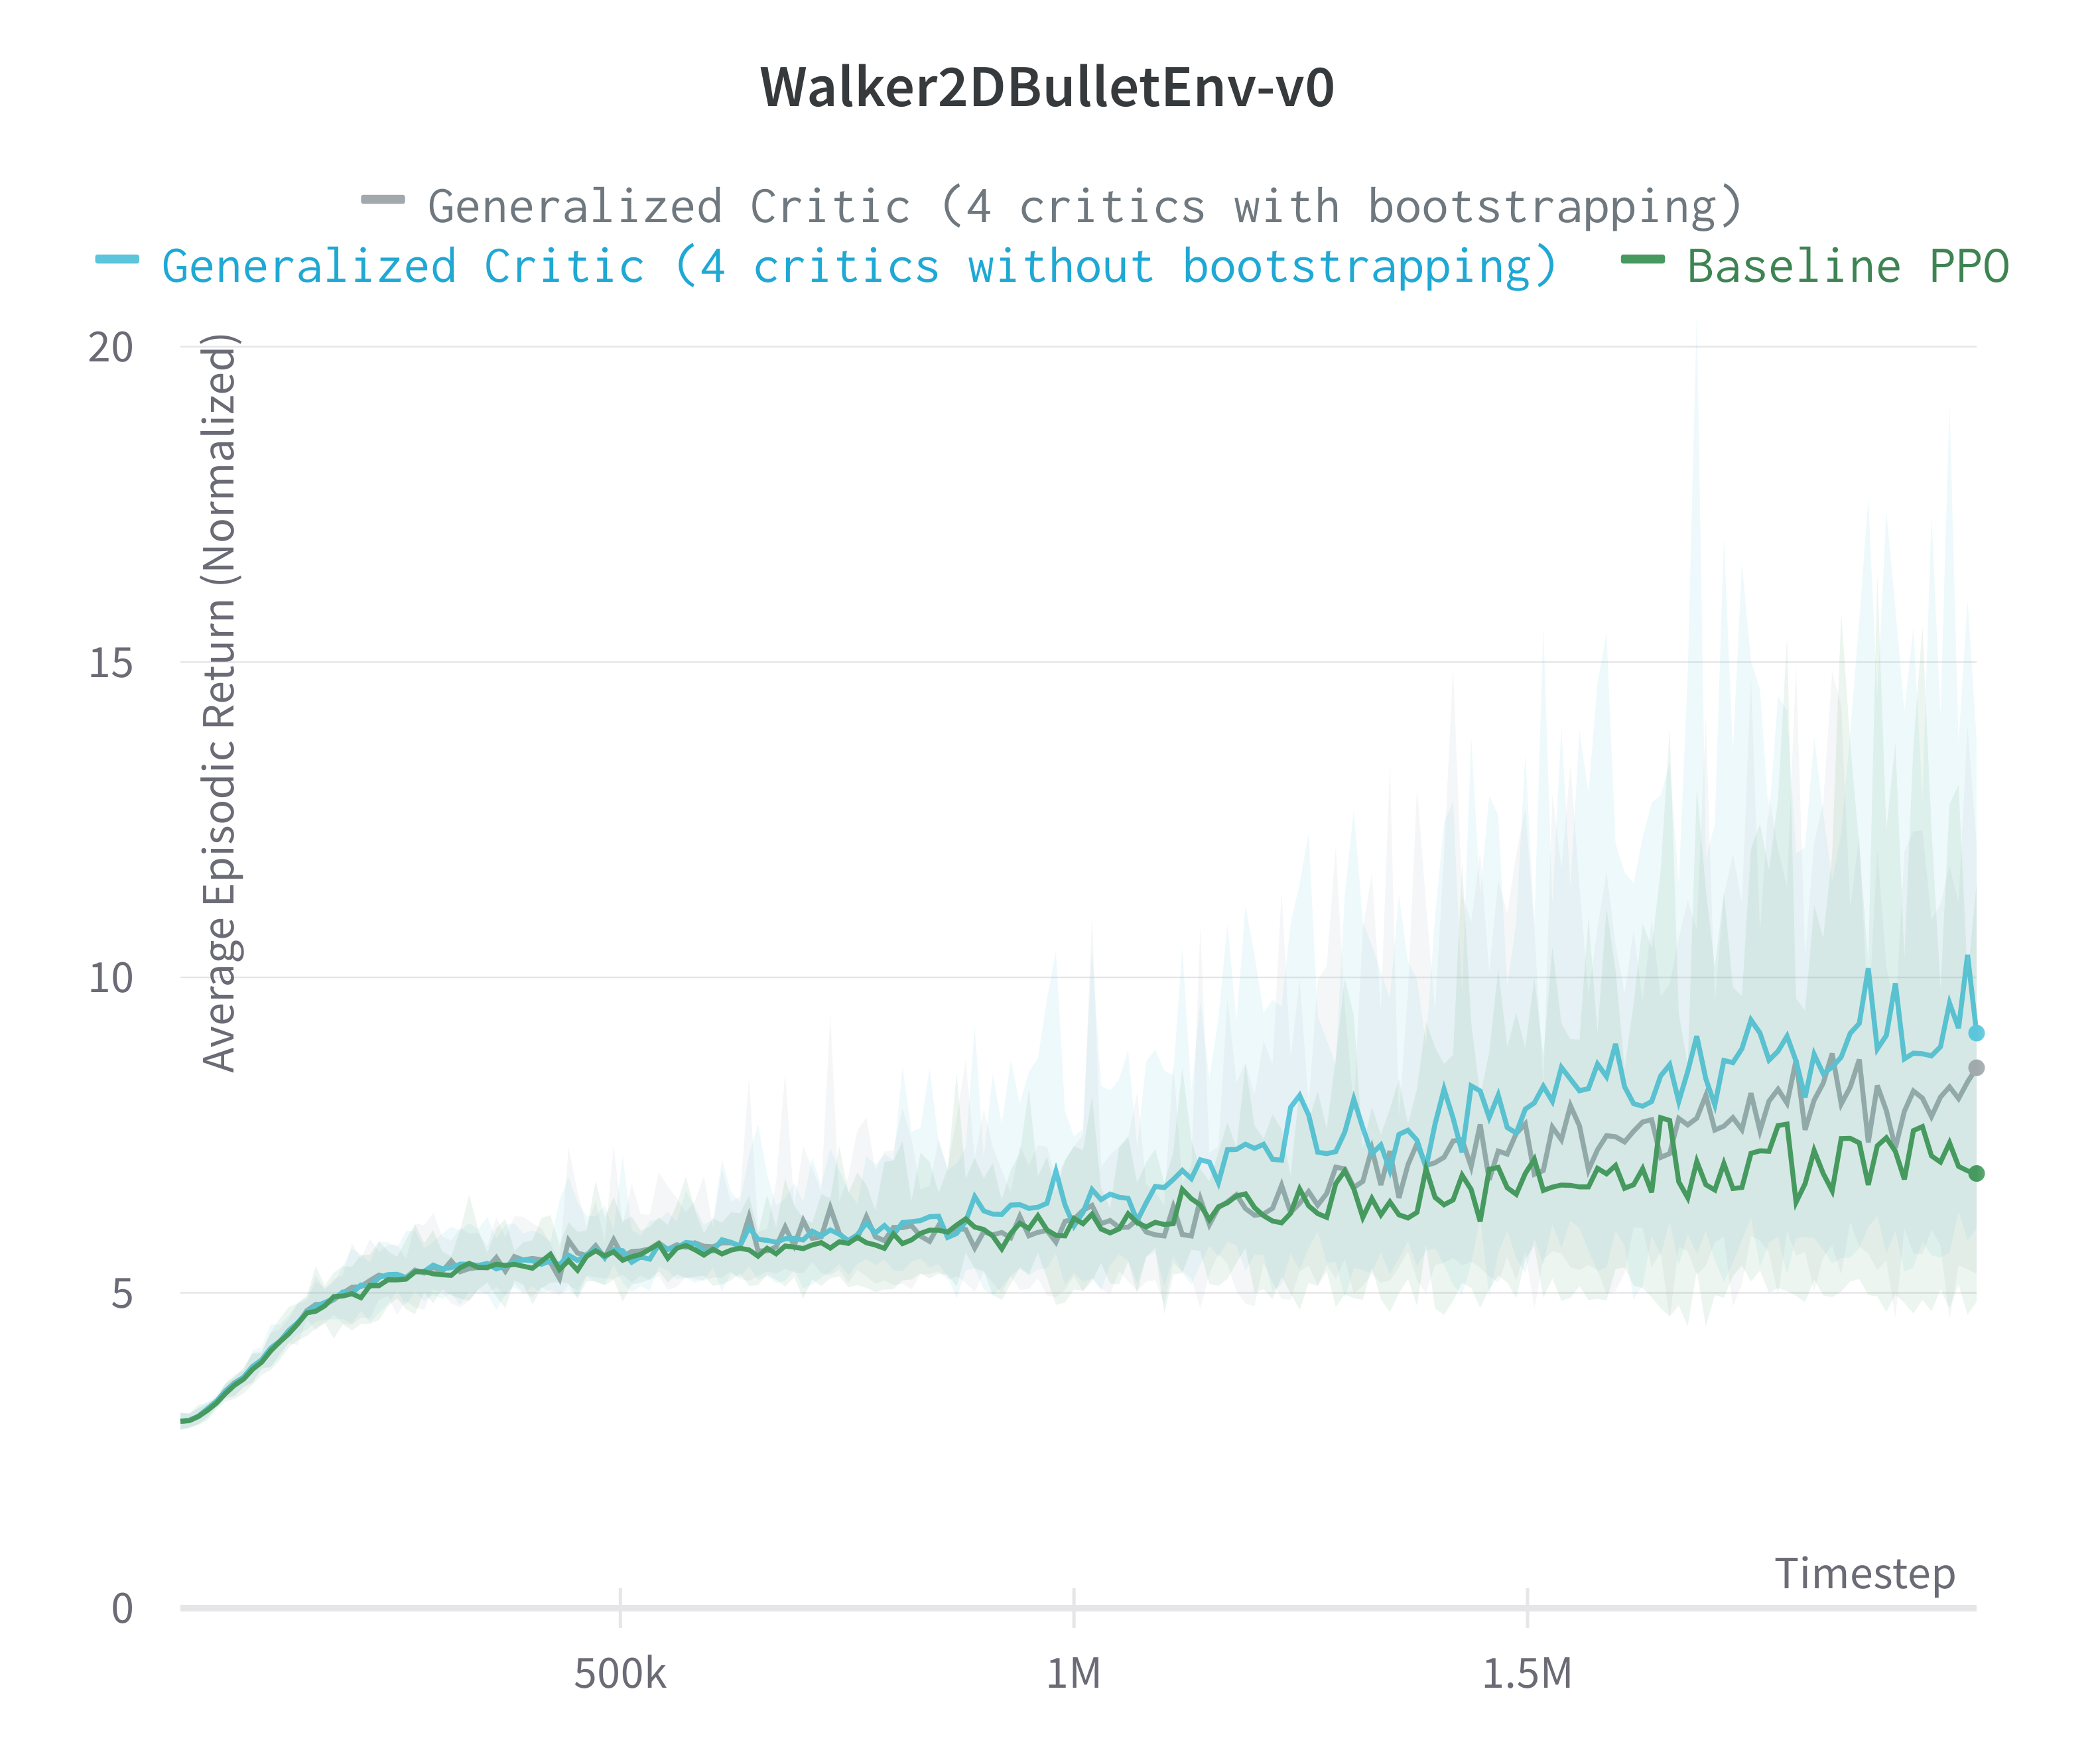
\includegraphics[width=\linewidth]{images/walker2D}}
%  \vspace{2.0cm}
%  \centerline{(a) Walker2DBulletEnv-v0}\medskip
\end{minipage}
\begin{minipage}[b]{.5\linewidth}
  \centering
  \centerline{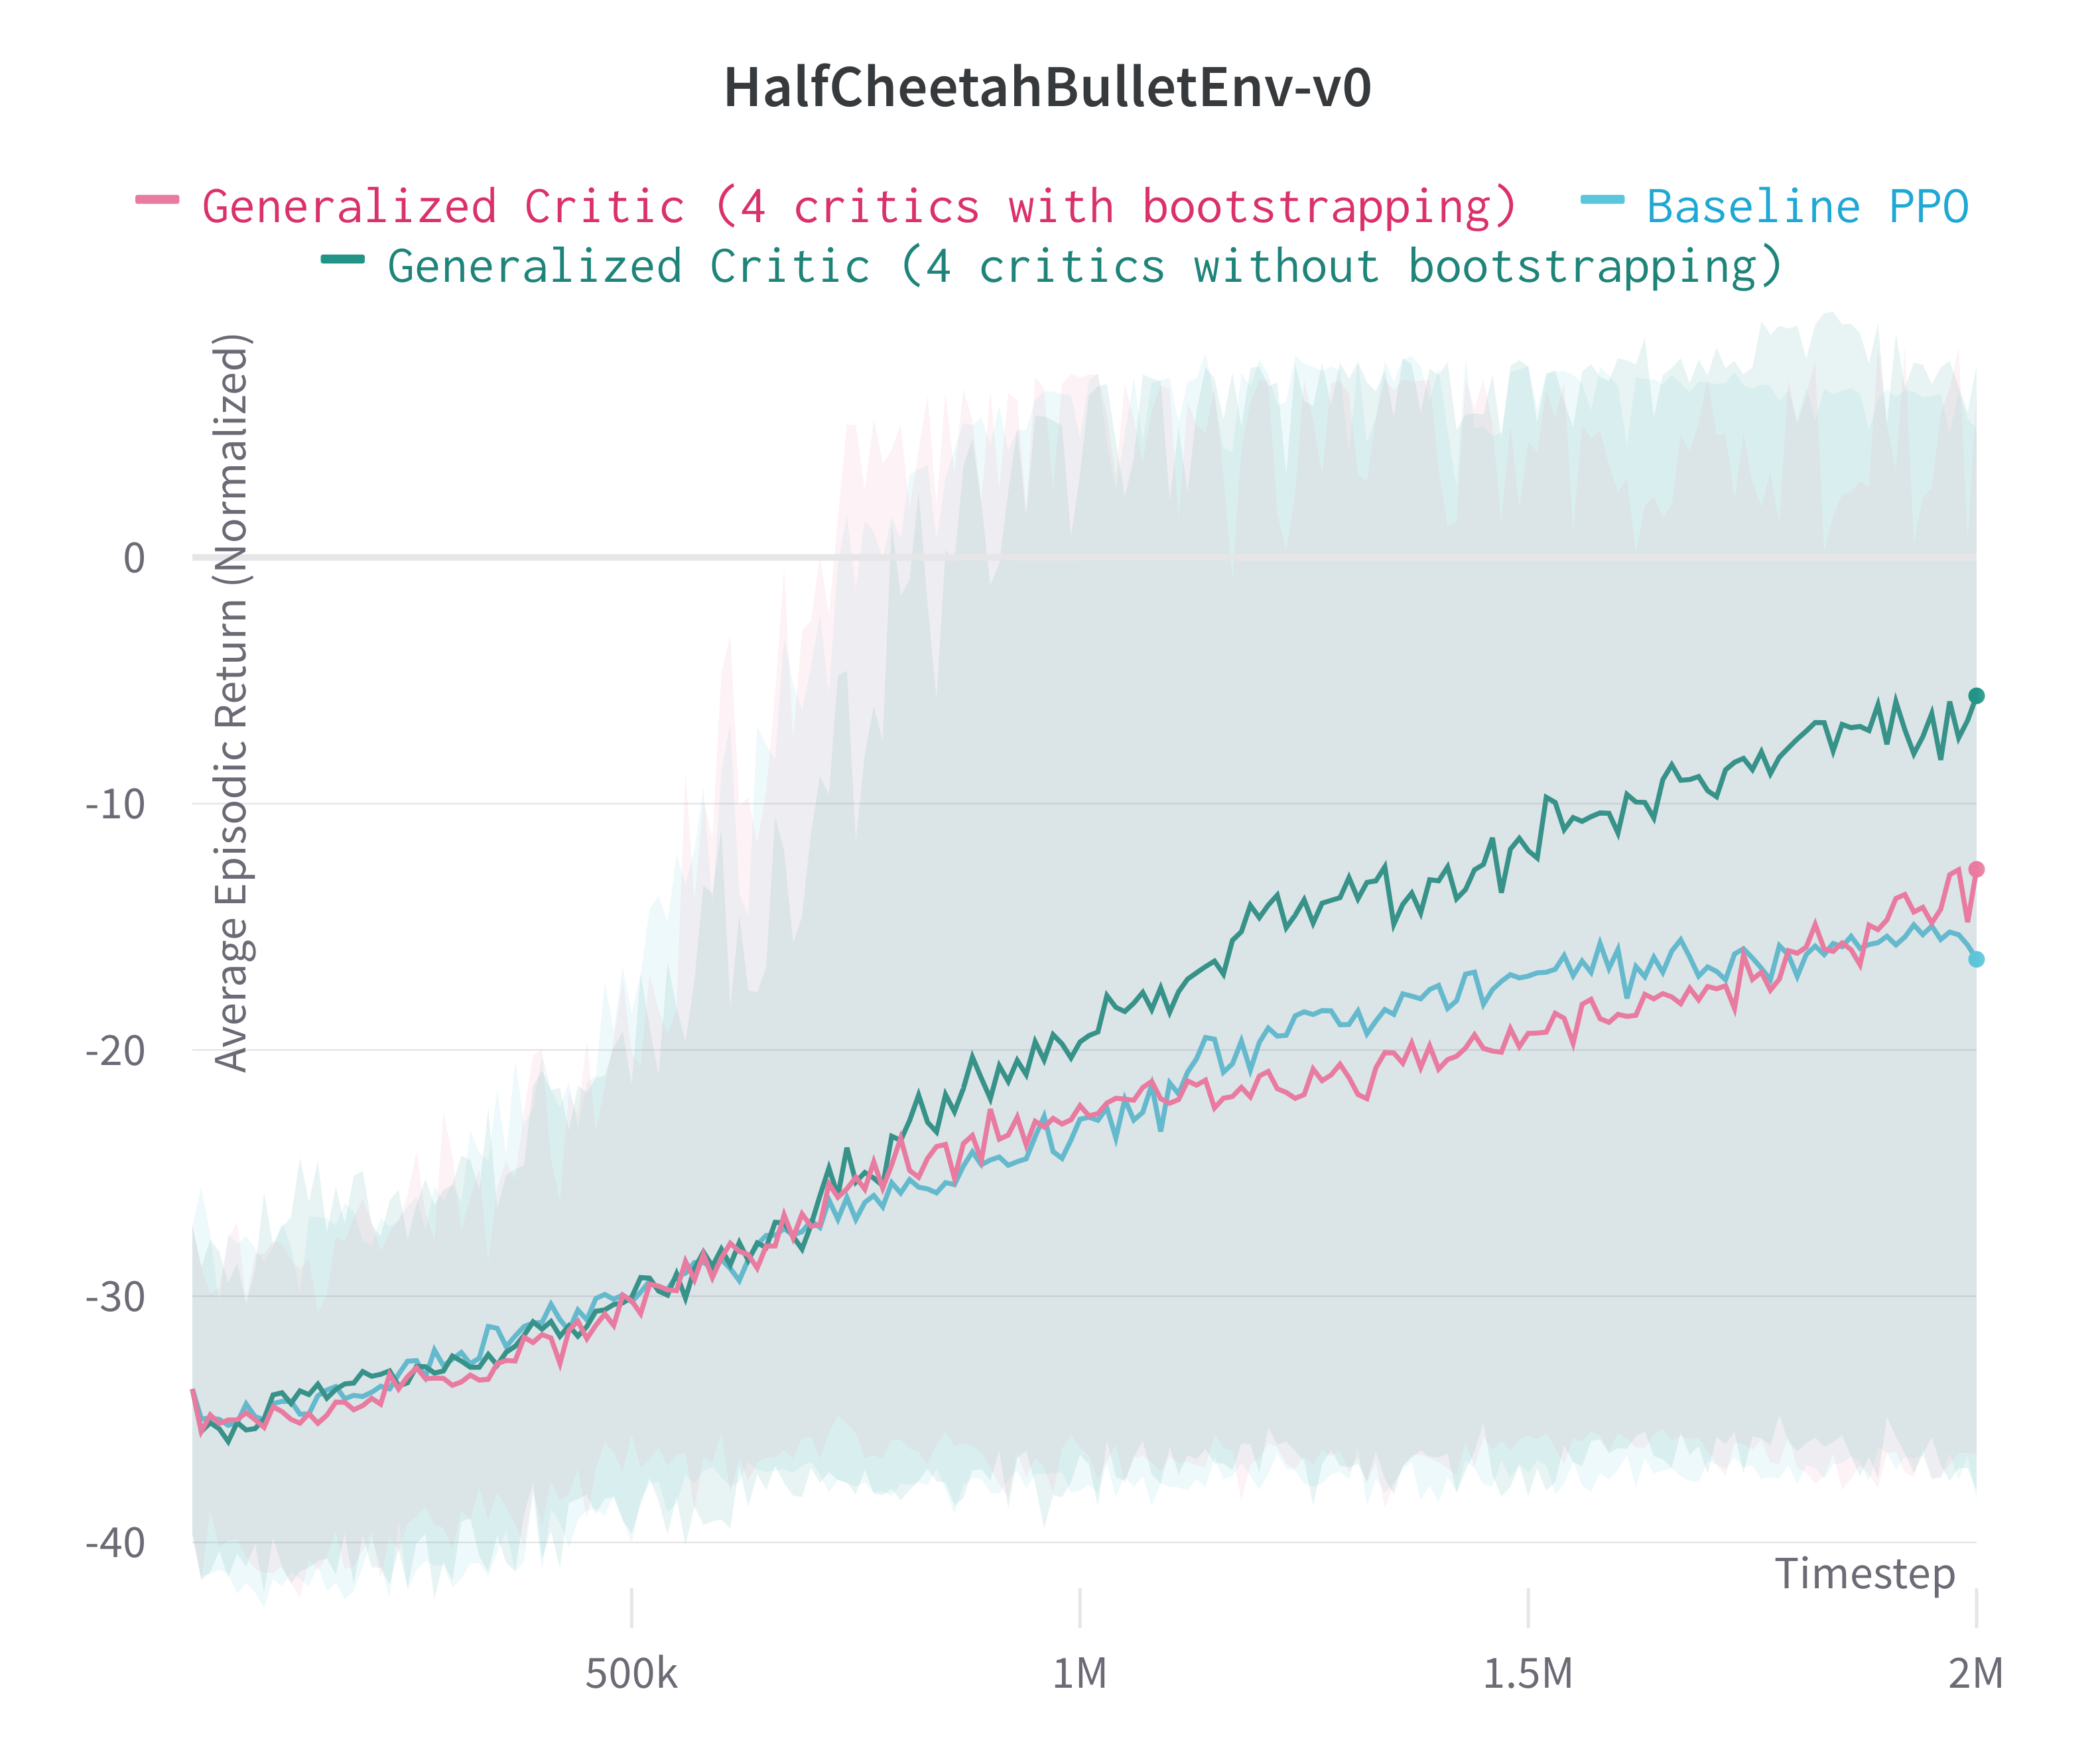
\includegraphics[width=\linewidth]{images/halfcheetah}}
%  \vspace{2.0cm}
%  \centerline{(b) HalfCheetahBulletEnv-v0}\medskip
\end{minipage}

\begin{minipage}[b]{.5\linewidth}
  \centering
  \centerline{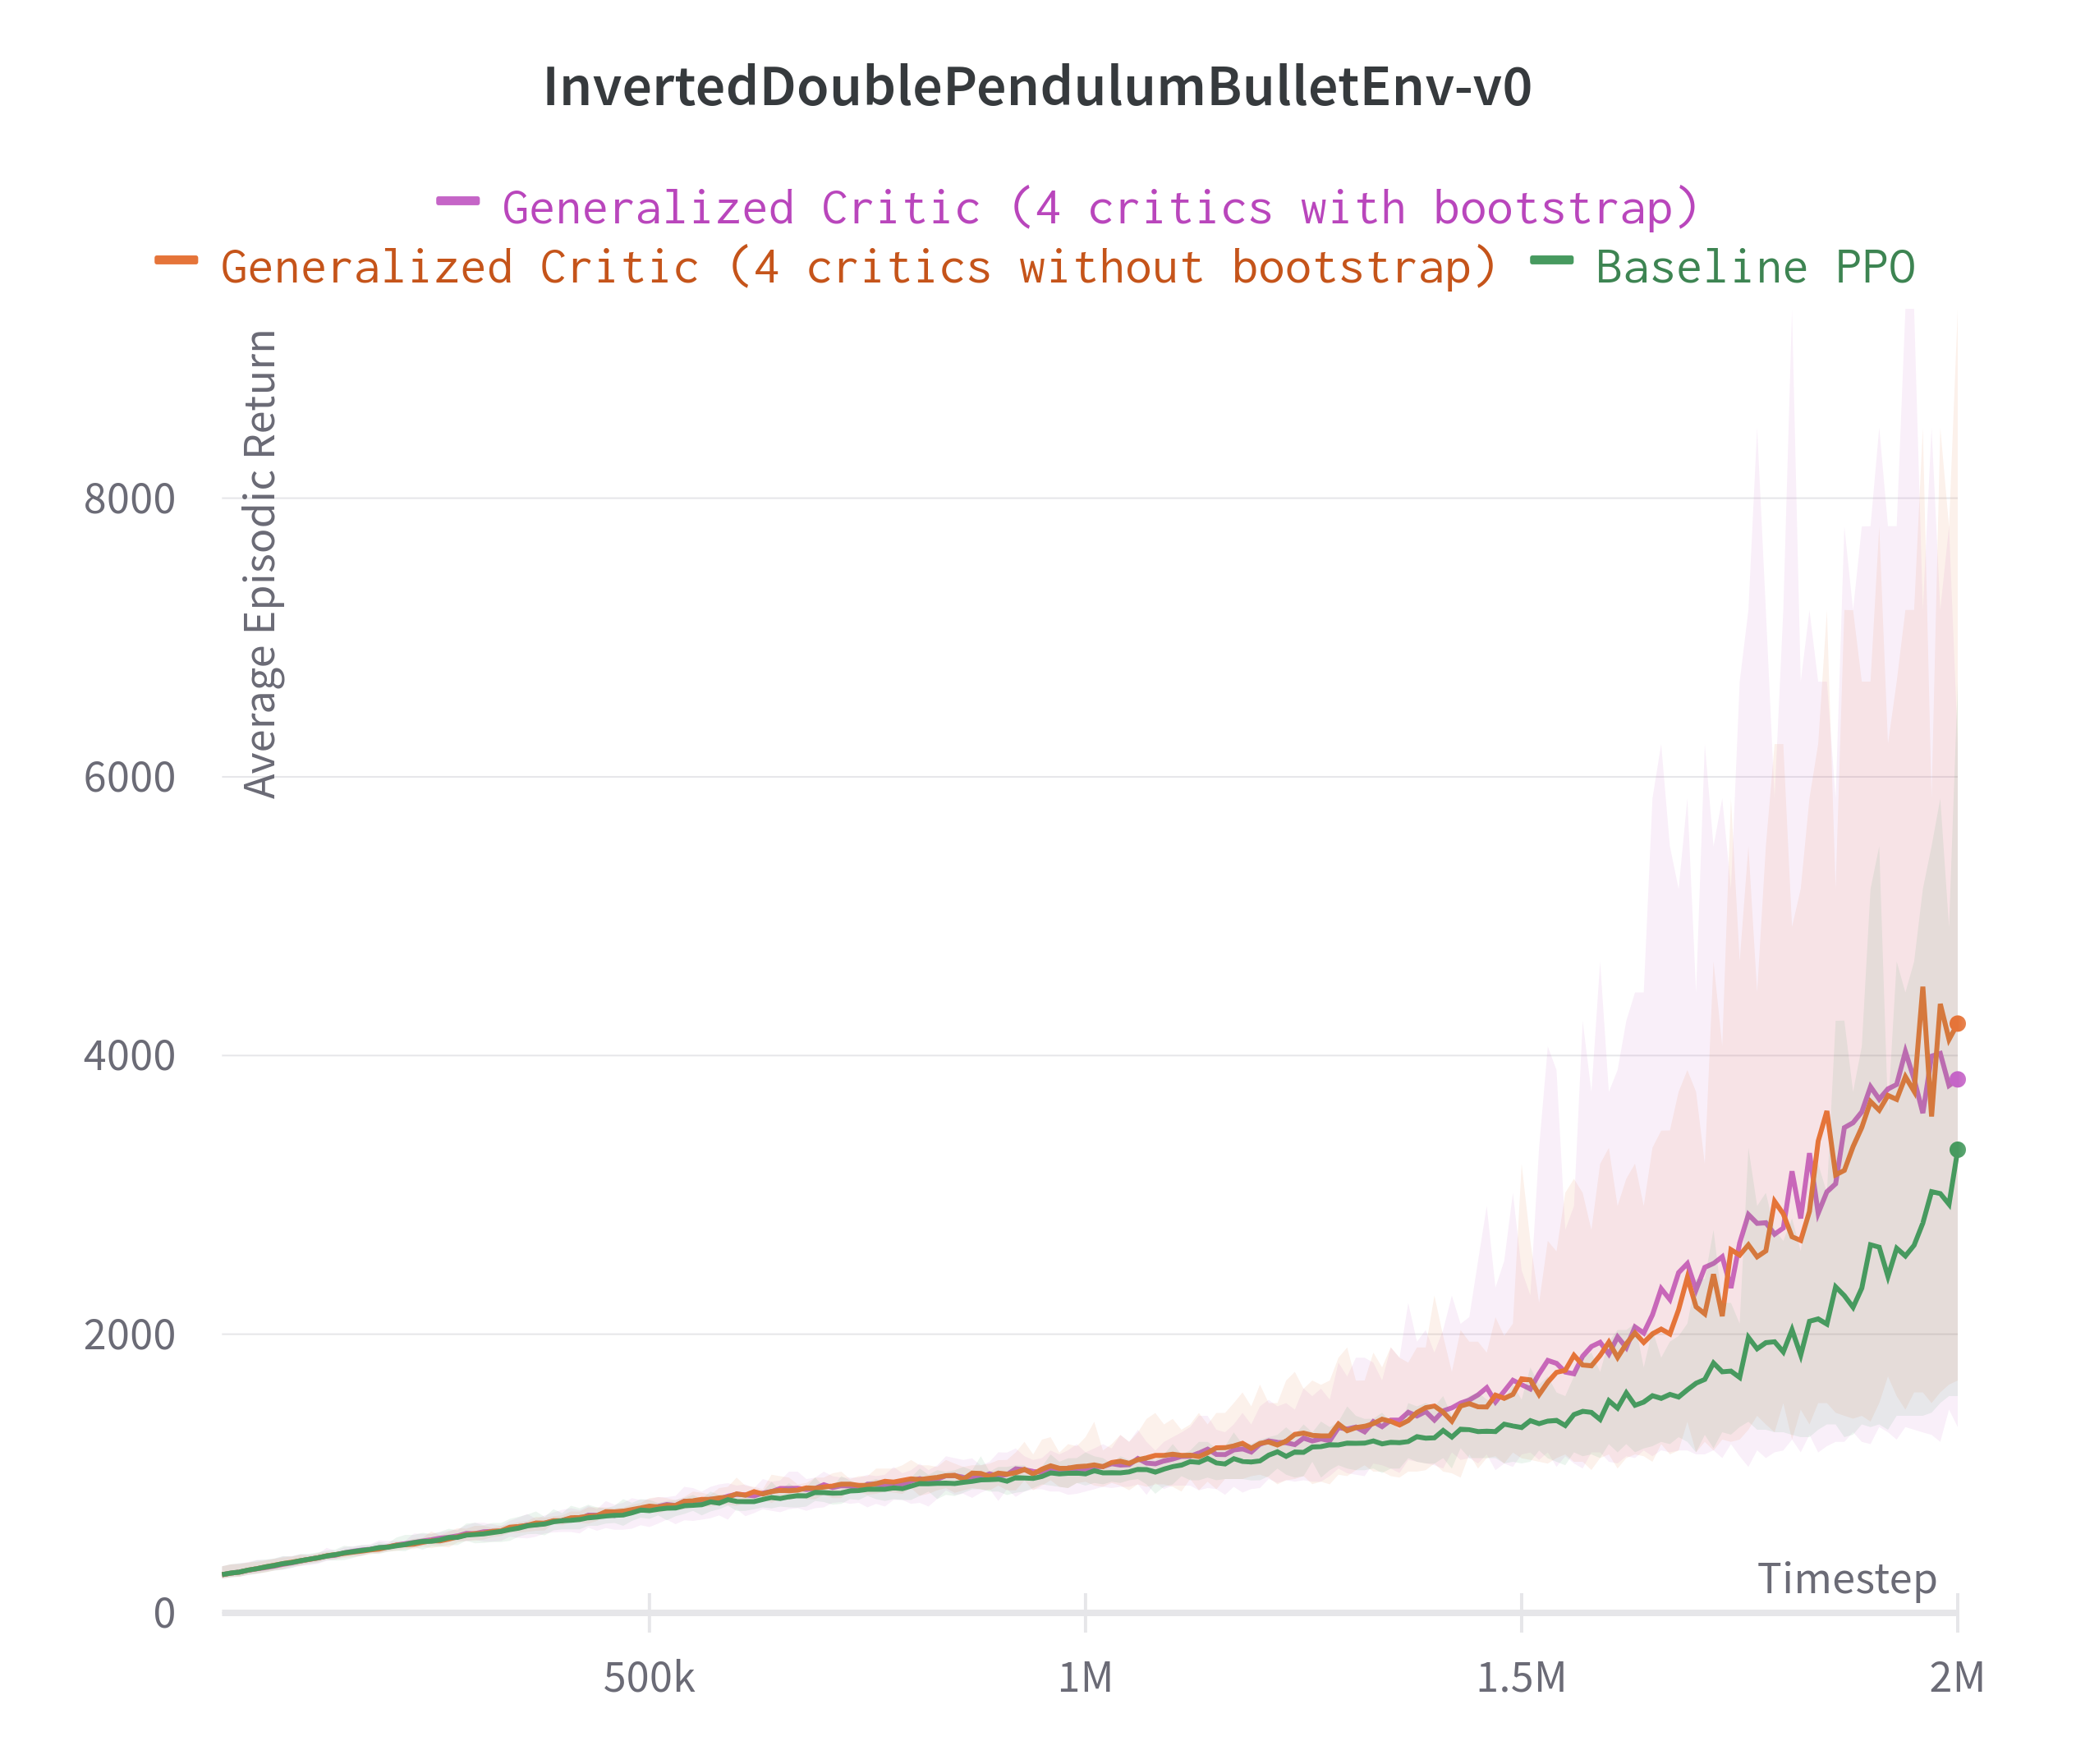
\includegraphics[width=\linewidth]{images/inverteddoublependulum}}
%  \vspace{2.0cm}
%  \centerline{(a) InvertedDoublePendulumBulletEnv-v0}\medskip
\end{minipage}
\begin{minipage}[b]{.5\linewidth}
  \centering
  \centerline{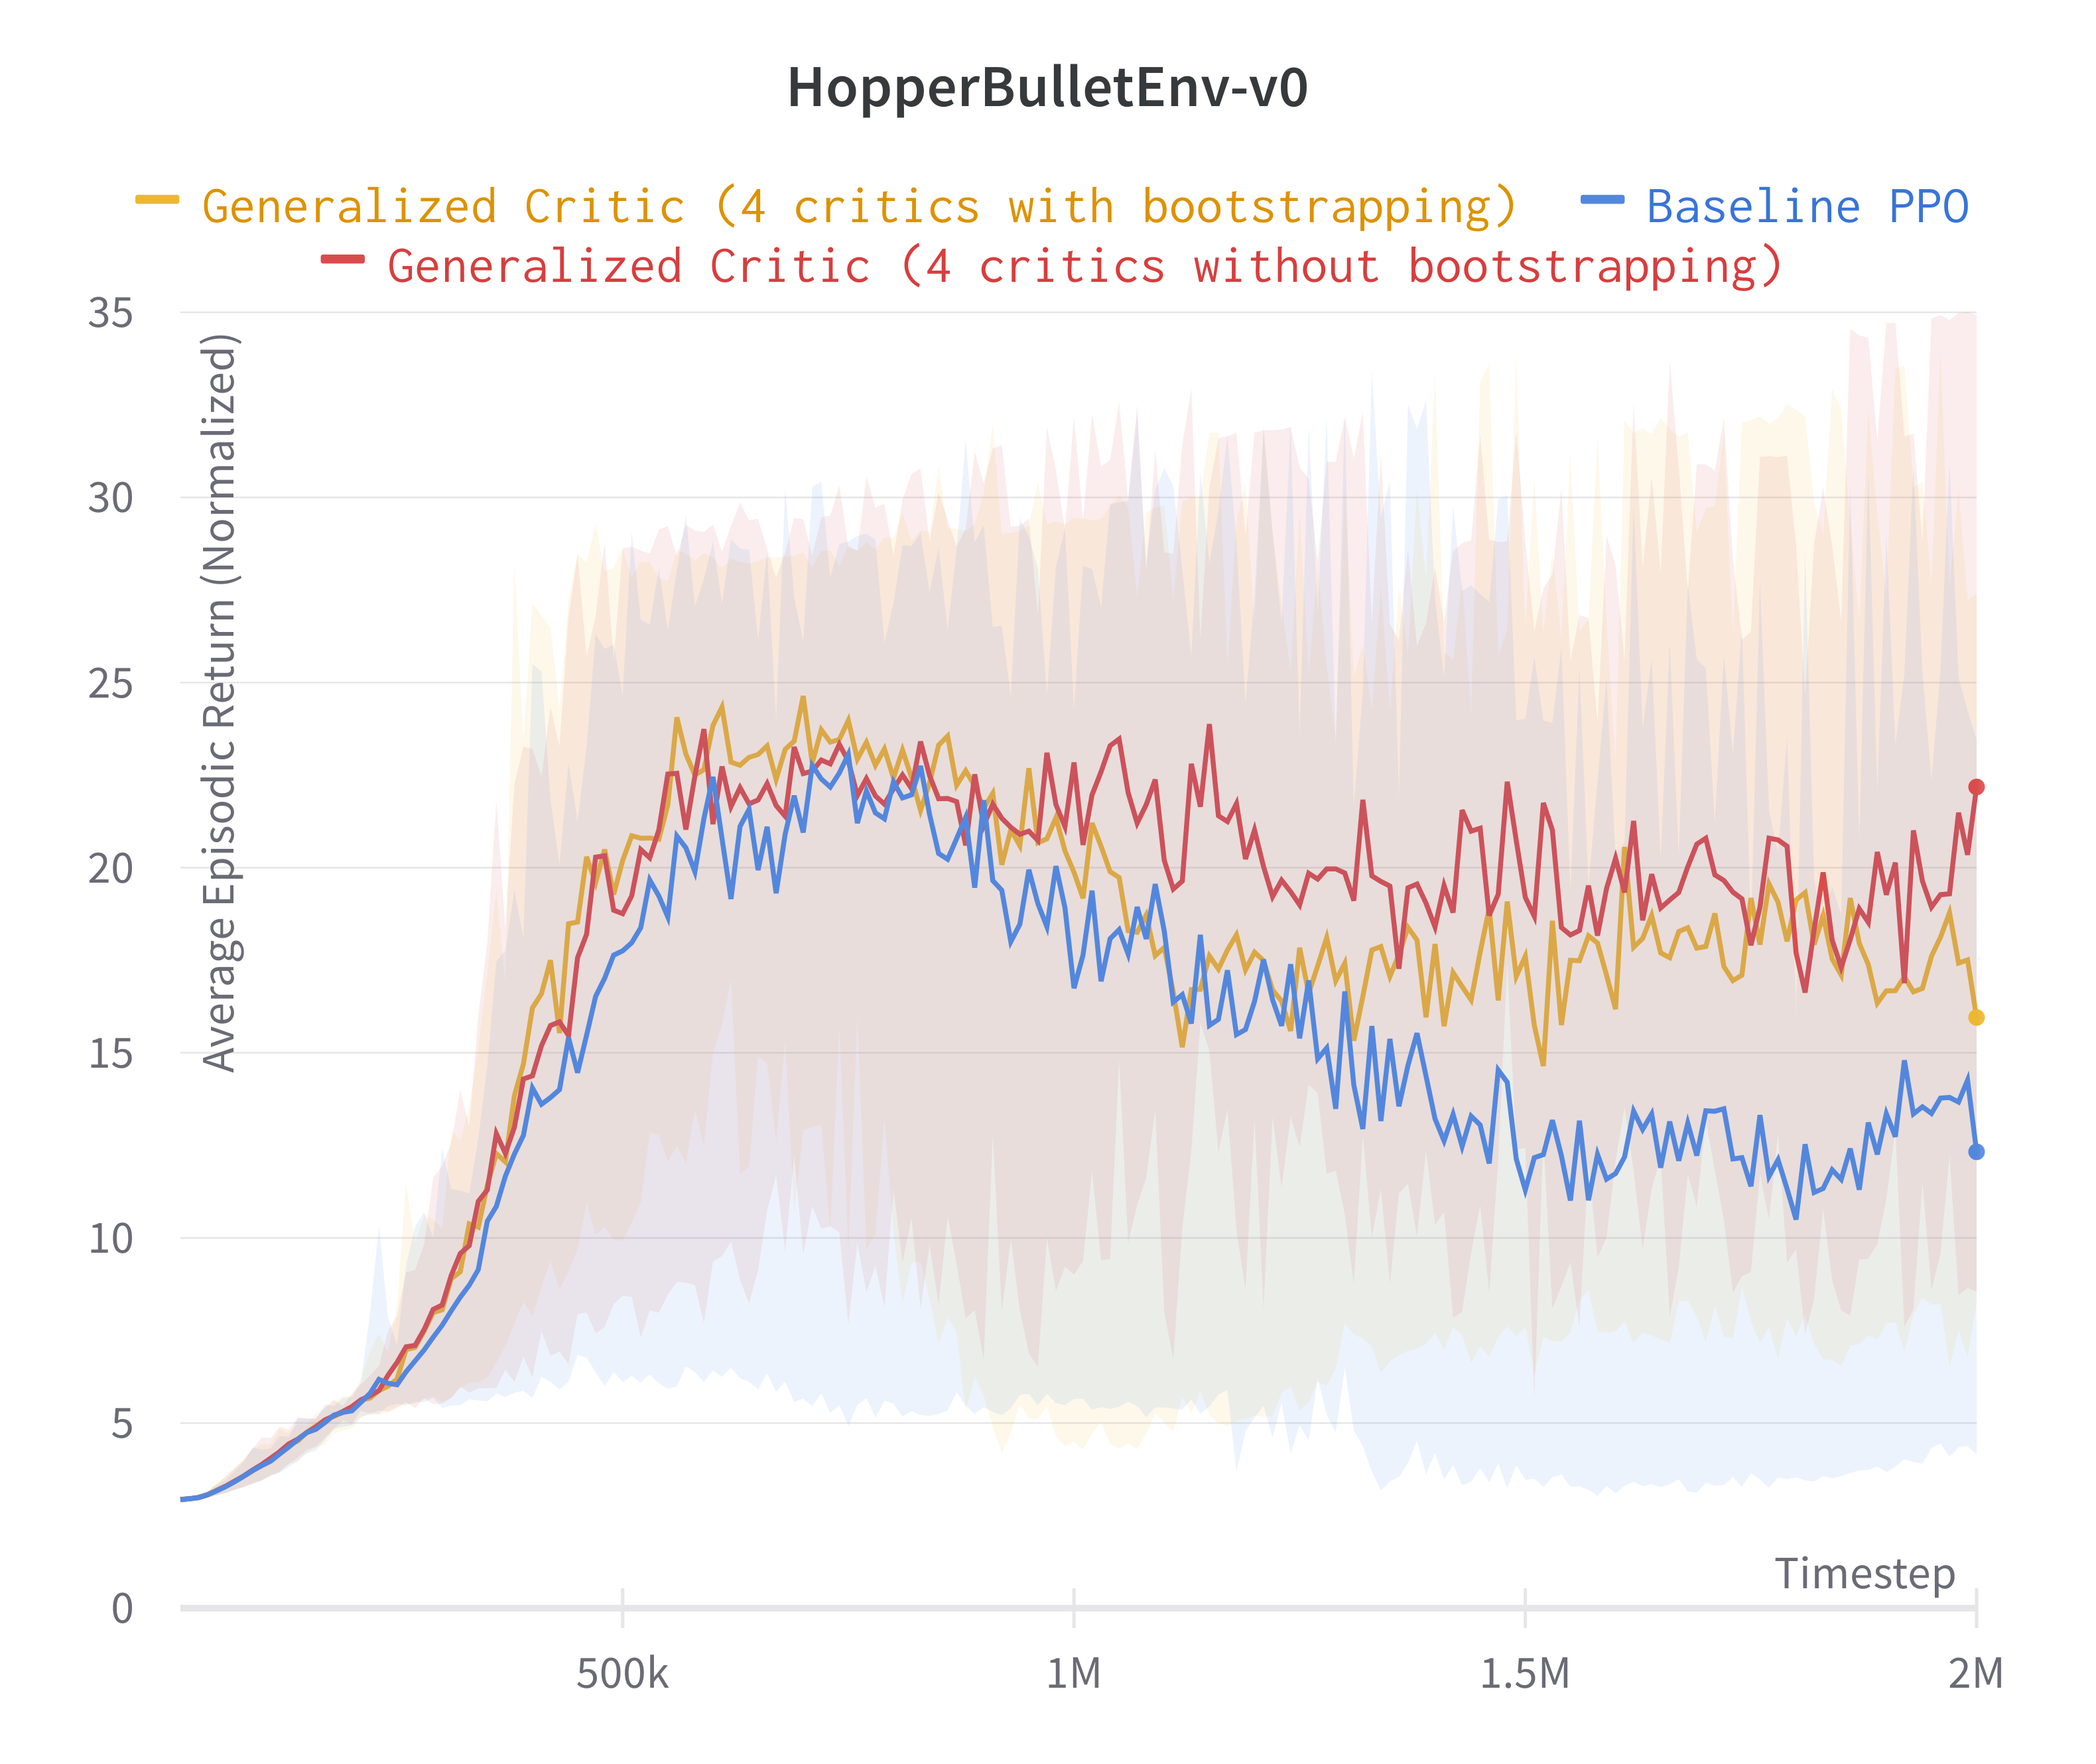
\includegraphics[width=\linewidth]{images/hopper}}
%  \vspace{2.0cm}
%  \centerline{(b) HopperBulletEnv-v0}\medskip
\end{minipage}
\caption{(2)}
\label{exp2}
\end{figure}
